\documentclass[serif, aspectratio=169]{beamer}
\usepackage[T1]{fontenc} 
\usepackage{fourier}
\usepackage{hyperref}
\usepackage{latexsym,amsmath,xcolor,multicol,booktabs,calligra}
\usepackage{graphicx,pstricks,listings,stackengine}
\usepackage{lipsum}
\usepackage{wrapfig}
\usepackage{url}
\usepackage{subcaption}

\usepackage{etoolbox}

\input{math_commands.tex}

\author{Yan Lin}
\title{AMDEN: Amorphous Materials DEnoising Network}
\subtitle{Generation of Amorphous Materials with Tailored Properties}
\institute{
    \href{mailto:lyan@cs.aau.dk}{lyan@cs.aau.dk}\\
    \href{https://www.en.tech.aau.dk/research/research-groups/data-engineering-science-og-systems-dess}{Data Engineering, Science and Systems} \\
    \href{https://www.en.aau.dk/}{Aalborg University} \\
}
\date{\small \today}
\usepackage{AAU}

% Remove navigation buttons
\setbeamertemplate{navigation symbols}{}

% defs
\def\cmd#1{\texttt{\color{red}\footnotesize $\backslash$#1}}
\def\env#1{\texttt{\color{blue}\footnotesize #1}}
% set colors
\definecolor{aauyellow}{RGB}{167, 131, 55}
\definecolor{aaublue}{RGB}{32, 26, 78}
\definecolor{aaured}{RGB}{152, 43, 28}

\def\emphasis#1{\color{aaured}#1}


\lstset{
    basicstyle=\ttfamily\small,
    keywordstyle=\bfseries\color{deepblue},
    emphstyle=\ttfamily\color{deepred},    % Custom highlighting style
    stringstyle=\color{deepgreen},
    numbers=left,
    numberstyle=\small\color{halfgray},
    rulesepcolor=\color{red!20!green!20!blue!20},
    frame=shadowbox,
}

%- --- --- --- --- --- --- --- --- --- --- --- --- --- --- --- 
\begin{document}

\begin{frame}
    \titlepage
    \vspace*{-0.6cm}
    \begin{figure}[htpb]
        \begin{center}
            \includegraphics[keepaspectratio, scale=0.5]{aau-logo-left-uk.pdf}
        \end{center}
    \end{figure}
\end{frame}

% \begin{frame}    
% \tableofcontents[sectionstyle=show,
% subsectionstyle=show/shaded/hide,
% subsubsectionstyle=show/shaded/hide]
% \end{frame}

\section{Background}

\begin{frame}{Discovery Amorphous Materials with Desired Properties}
    \begin{block}{Trial-and-error}
        Screen through the design space until samples with desired properties is found.

        \begin{figure}[htpb]
            \vspace{-0.3cm}
            \begin{center}
                \includegraphics[keepaspectratio, height=0.25\textheight]{figures/screen.pdf}
            \end{center}
            \vspace{-0.3cm}
        \end{figure}
    \end{block}

    \begin{block}{Inverse Design}
        Begin with desired properties and generate the atomic configurations to achieve them.
        \begin{figure}[htpb]
            \vspace{-0.3cm}
            \begin{center}
                \includegraphics[keepaspectratio, height=0.25\textheight]{figures/generation.pdf}
            \end{center}
            \vspace{-0.3cm}
        \end{figure}
    \end{block}
\end{frame}


\begin{frame}{Generative Modeling of Amorphous Materials}
    Start from a initial state of the sample, adjust its atomic positions and elements step-by-step towards the final state.
    \begin{itemize}
        \item Similar to a simulation pipeline but the atoms are not driven by energy and force
        \item Instead, a \textit{neural network} predicts the movements of atoms at each step conditioned on the desired properties
    \end{itemize}
    \begin{figure}
        \centering
        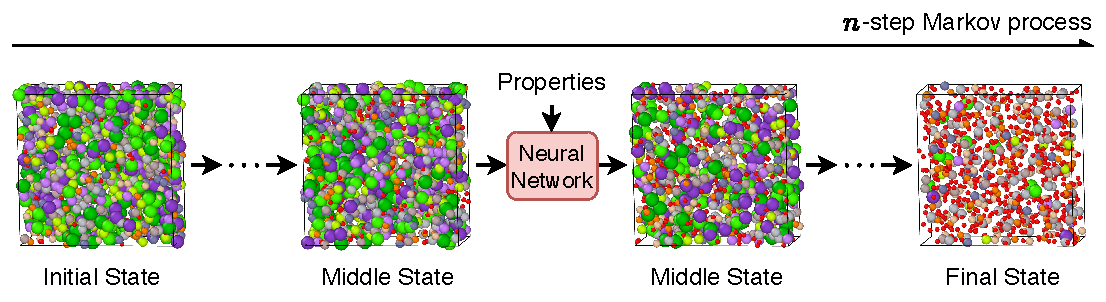
\includegraphics[width=\linewidth]{figures/process.pdf}
    \end{figure}
\end{frame}


\section{Problem}

\begin{frame}{Neural Network for Generative Modeling}
    \begin{itemize}
        \item Input: Current state of an amorphous material sample at each step, and the desired properties
        \item Output: State of the sample at next step
    \end{itemize}
    \begin{figure}
        \centering
        \includegraphics[width=.8\linewidth]{figures/network-problem.pdf}
    \end{figure}
\end{frame}

\begin{frame}{Reversable Generation Process}
    We cannot train a neural network with the generation process alone.

    \begin{figure}
        \centering
        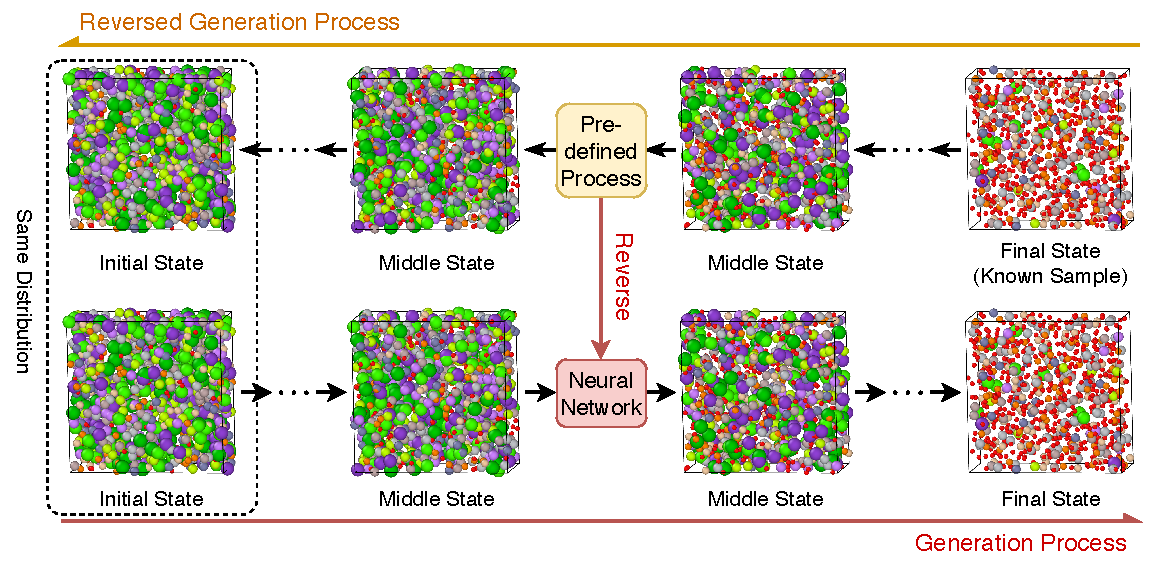
\includegraphics[width=.8\linewidth]{figures/reverse-process.pdf}
        \vspace{-0.3cm}
    \end{figure}

    A reversed generation process providing ground truth for training.
\end{frame}


\section{Methodology}

\begin{frame}{Representation of Amorphous Material Samples}
    \begin{columns}
        \begin{column}{0.6\textwidth}
            Representing one amorphous material sample as a tuple $x=(\mC, \mX, \mE)$.

            \begin{itemize}
                \item $\mC \in \mathbb R^{3\times 3}$ is the lattice vectors
                \item $\mX \in \mathbb R^{N\times 3}$ is the atomic positions
                \item $\mE \in \mathbb R^{N\times d}$ is the element one-hot embeddings
            \end{itemize}

            And its properties as a vector $\vy$ where each value is a scalar property.
        \end{column}
        \begin{column}{0.4\textwidth}
            \begin{figure}
                \centering
                \includegraphics[width=\linewidth]{figures/sample-rep.pdf}
            \end{figure}
        \end{column}
    \end{columns}
\end{frame}

\begin{frame}{Equivalent Neural Network Architecture}
    Preserve the geometric equivariance of amorphous material samples.
    \begin{figure}
        \centering
        \includegraphics[width=\linewidth]{figures/network.pdf}
    \end{figure}

    \begin{itemize}
        \item A graph structure of each sample where node and edge features are invariant to permutation and translation
        \item EGNN\footnote{Satorras, Vıctor Garcia, Emiel Hoogeboom, and Max Welling. "E (n) equivariant graph neural networks." International conference on machine learning, 2021.} backbone whose update to each sample is invariant
    \end{itemize}
\end{frame}

\begin{frame}{Denoising Generation Process}
    \begin{itemize}
        \item The reversed generation process gradually add Gaussian noise to the sample until the pure noise at initial state
        \item The neural network learns to remove the noise added in each step
        \item The generation process can start from a initial state of pure Guassian noise
    \end{itemize}

    \begin{figure}
        \centering
        \includegraphics[width=.8\linewidth]{figures/denoising.pdf}
    \end{figure}
\end{frame}


\section{Results}
\begin{frame}{Generation of Amorphous Silica}
    With desired shear modulus and average ring size that are dependent on the samples' structures and densities.

    \begin{figure}
        \centering
        \begin{subfigure}{0.45\textwidth}
            \centering
            \includegraphics[width=\linewidth]{figures/SiO2-G.pdf}
            \caption{Accuracy of shear modulus of generated samples}
        \end{subfigure}
        \hfill
        \begin{subfigure}{0.45\textwidth}
            \centering
            \includegraphics[width=\linewidth]{figures/SiO2-RSD.pdf}
            \caption{Accuracy of average ring size of generated samples}
        \end{subfigure}
    \end{figure}
\end{frame}

\begin{frame}{Generation of Multi-element Glass}
    With desired Young's modulus and Lithium ratio that are largely dependent on samples' compositions.

    \begin{figure}
        \centering
        \begin{subfigure}{0.45\textwidth}
            \centering
            \includegraphics[width=\linewidth]{figures/bmp_E.pdf}
            \caption{Accuracy of Young's modulus of generated samples}
        \end{subfigure}
        \hfill
        \begin{subfigure}{0.45\textwidth}
            \centering
            \includegraphics[width=\linewidth]{figures/bmp_Li.pdf}
            \caption{Distribution of Lithium ratio of training data and generated samples (with target being 0.15)}
        \end{subfigure}
    \end{figure}
\end{frame}

\begin{frame}{Limitations}
    \begin{block}{Real-world synthesis of generated samples}
        New synthesis techniques is needed to fully take advantage of the generated atomic configurations.
    \end{block}

    \begin{block}{Generation of samples with relaxed structures}
        Unable to generate amorphous materials with relaxed structures, an inherent limitation of such prediction-based generative model.
    \end{block}

    \vspace{1em}
    \textbf{Further discussion and solutions: stay tuned for the next session!}
\end{frame}


\begin{frame}
\begin{center}
{\large Thank you!}
\vspace{1cm}
\\[0.5em]
{\small \href{mailto:lyan@cs.aau.dk}{lyan@cs.aau.dk} \\
\href{www.yanlincs.com}{www.yanlincs.com}}
\end{center}
\end{frame}

\end{document}
